% Sole manuscript source. The legacy filename remains the Overleaf root.
\documentclass{article}
\PassOptionsToPackage{table}{xcolor}
\usepackage{iclr2027_conference,times}
\usepackage[T1]{fontenc}
\usepackage[utf8]{inputenc}
\usepackage{amsmath,amssymb,amsthm,booktabs,multirow,adjustbox}
\usepackage{xcolor}
\usepackage{enumitem,graphicx,microtype,url,hyperref}
\hypersetup{hidelinks}
\newtheorem{proposition}{Proposition}
\newtheorem{corollary}[proposition]{Corollary}
\newcommand{\pre}{\mathrm{pre}}
\newcommand{\off}{\mathrm{off}}
\newcommand{\cross}{\mathrm{cross}}
\newcommand{\diag}{\operatorname{diag}}
\newcommand{\op}[1]{\left\|#1\right\|_2}
\newcommand{\fro}[1]{\left\|#1\right\|_F}
\newcommand{\allocationbar}[4]{\makebox[1em][l]{#1}\begingroup\setlength{\unitlength}{\dimexpr\linewidth-1em\relax}\textcolor{black!80}{\rule{#2\unitlength}{1.4ex}}\textcolor{black!45}{\rule{#3\unitlength}{1.4ex}}\textcolor{black!15}{\rule{#4\unitlength}{1.4ex}}\endgroup}
\title{Confinement, Flexibility, and Mixing\\in Spectral Fine-Tuning}
\author{Anonymous authors}
% Keep anonymous; do not enable \iclrfinalcopy for submission.
\begin{document}
\maketitle

\begin{abstract}
What does a spectral constraint preserve during fine-tuning? We distinguish confinement to a pretrained singular subspace, suppression of interaction between subspaces, and stability of the top-ranked singular directions. Using fixed tail coefficients, within-tail rotations, and ambient diagonal scalers as experimental instruments, we characterize two approximation bottlenecks and derive mixing bounds with and without a leading core. A projector-commutator characterization shows that the scaler penalty suppresses nonuniformity, motivating a distinction between frame-specific effects and generic regularization. In archived RoBERTa-base runs on five tasks, unregularized leading/cross/tail energy shares lie near a dimension-only reference. Two-sided regularization lowers cross energy from approximately 43\% to 10--27\%, yet leaves 44--64\% in the leading block. These changes accompany 5--9-fold smaller task-mean relative update norms; score changes vary by seed, with task-mean decreases of roughly $0.2$--$1.0$ points. This descriptive result separates block decoupling from tail confinement, but does not identify a benefit beyond shrinkage or scaler homogenization. Supporting GLUE and generation results demonstrate task learning, with substantial frozen-basis storage and unmerged computation. Spectral preservation must therefore specify the object preserved, not just the penalty applied.
\end{abstract}
\section{Introduction}
\label{sec:intro}

Parameter-efficient fine-tuning (PEFT) adapts a pretrained model through a restricted set of trainable parameters. Rank, parameter count, and task performance are natural descriptions of these restrictions, but they leave an important question open: where does the effective update lie relative to the structure of the pretrained weights? Two updates can have the same rank and magnitude while modifying different pretrained directions. Likewise, similar downstream performance need not imply similar spectral changes, as studies comparing LoRA and full fine-tuning demonstrate~\citep{hu2022lora,shuttleworth2025illusion}.

The singular value decomposition of a pretrained weight matrix provides a fixed reference for this question. Its leading and tail singular subspaces define a partition of the update into leading--leading, tail--tail, and two cross blocks. This is a geometric distinction, not a semantic assignment: a large singular value does not by itself identify stored knowledge, and a small singular value does not identify dispensable noise. The reference frame instead lets us ask what a constraint preserves, what freedom it removes, and how a relaxation interacts with the original directions.

This reference frame is already used by spectral fine-tuning methods, including singular-value tuning, singular-vector coefficient tuning, and regularized adaptation of singular factors~\citep{han2023svdiff,lingam2024svft,cao2025sorsa}. Our question is not whether pretrained spectral information can be used for adaptation, but what different uses of that information actually constrain. In particular, orthonormality of trainable factors, confinement to a pretrained subspace, and stability of the largest singular directions are different properties.

We investigate a hierarchy of constraints: fixed tail coefficients, within-tail rotations, and ambient diagonal scalers. Their implementation labels are LinLoRA, OrthoLoRA, UILinLoRA, and UIOrthoLoRA. The historical prefix UI means ``unit-invariant''; here it identifies learned coordinate scalers, not a proved invariance property. These constructions are instruments for comparing constraints, not contenders for a best-adapter claim. The practical scaled update need not be low-rank despite the legacy suffix.

The analysis yields two separations. First, exact projection identities distinguish an outside-tail approximation residual from the additional error imposed by a diagonal tail core. They hold for any target perturbation, without assuming that task-relevant directions align with the tail. Second, the meaning of mixing control depends on the core being scaled. A tail-only core recovers confinement when mixing vanishes. A practical leading-plus-tail core instead permits direct leading adaptation even when its cross blocks vanish. Thus suppressing mixing need not preserve the leading weight block, and preserving that block need not preserve its rank ordering after adaptation.

Across five GLUE tasks, penalizing both scaler mixing operators reduces cross energy from approximately 43\% to 10--27\% and increases tail allocation. Yet the leading block's share rises in four of five task means. Aggregate off-tail leakage would hide this distinction. The same intervention shrinks updates substantially, while one-sided regularization achieves the highest mean task scores on three tasks without comparable cross suppression. These endpoints establish co-occurring geometric and functional changes, not a necessary geometry--performance trade-off or a magnitude-independent effect.

Our contributions are the separation of within-span and outside-span bottlenecks, unified bounds distinguishing confinement from decoupling, and a reproducible analysis of scaler regularization through effective update blocks. The central lesson is that lower cross interaction can coexist with a substantial leading modification. Establishing why this occurs requires separating the pretrained frame from generic scaler homogenization, initialization, and update magnitude.
\section{PEFT in pretrained singular coordinates}
\label{sec:coordinates}

For clarity, the main derivations use a square adapted matrix $W_0\in\mathbb R^{d\times d}$, as in the RoBERTa attention projections studied here. Let
\begin{equation}
W_0=U\Sigma V^\top
=U_L\Sigma_L V_L^\top+U_T\Sigma_T V_T^\top
\label{eq:pretrained}
\end{equation}
be a complete SVD with singular values in descending order. A declared cutoff $1\le k<d$ selects the leading $k$ directions, and the remaining $r=d-k$ directions form the tail. The cutoff is not the numerical rank: $\Sigma_T$ generally contains nonzero pretrained singular values. The pretrained weight $W_0$, including this tail, remains frozen. We define the effective update by $\Delta=W_{\mathrm{eff}}-W_0$ and its coordinates by
\begin{equation}
C=U^\top\Delta V=
\begin{bmatrix}C_{LL}&C_{LT}\\C_{TL}&C_{TT}\end{bmatrix}.
\label{eq:coordinates}
\end{equation}
Here $C_{LL}$ modifies the leading block, $C_{TT}$ acts within the tail, and $C_{LT},C_{TL}$ couple the two coordinate groups. We use \emph{cross mixing} for the last two blocks and \emph{off-tail allocation} for all three blocks outside $TT$. These terms are not interchangeable.

Orthogonal invariance and the disjoint blocks give
\begin{equation}
\fro{\Delta}^2=\fro{C}^2=\sum_{a,b\in\{L,T\}}\fro{C_{ab}}^2.
\label{eq:energy}
\end{equation}
For a nonzero update define $p_{ab}=\fro{C_{ab}}^2/\fro{\Delta}^2$, $p_{\cross}=p_{LT}+p_{TL}$, and $p_{\off}=p_{LL}+p_{\cross}$. The experiments report the off-tail \emph{norm ratio}, $q_{\off}=\sqrt{p_{\off}}$, and the relative magnitude $\rho_F=\fro{\Delta}/\fro{W_0}$. A mean of norm ratios cannot be squared to obtain the mean energy fraction. Absolute norms, normalized placement, and the aggregation across matrices must therefore be stated separately.

\paragraph{A common reference, not a method-specific score.}
This standard change of coordinates is compatible with singular-subspace perturbation analysis~\citep{wedin1972perturbation} and can measure any effective update. For LoRA, $\Delta=XY^\top$ gives $C_{ab}=(U_a^\top X)(V_b^\top Y)^\top$: low rank alone zeros none of the four blocks. This is an algebraic comparison; our block measurements below concern the spectral instruments. Block energies are invariant to within-subspace basis changes, but a diagonal coefficient family depends on the paired basis. Ties across the cutoff require one fixed declared reference. Rectangular complements are treated in Appendix~\ref{app:rectangular}. When insertion changes the initial effective matrix, displacement from $W_0$ and displacement since insertion are different quantities.

\paragraph{Structural change versus functional change.}
The coordinates describe weights. Leading-subspace drift additionally compares the top-ranked singular subspaces of $W_0$ and $W_0+\Delta$. Even a perfectly confined update can change that ranking if adapted tail singular values cross the boundary. Functional retention is a further question requiring behavior-level measurements; it does not follow from an unchanged block alone.
\section{Confinement and flexibility}
\label{sec:confinement}

\begin{figure}[t]
\centering
%
\begin{tabular}{cc}
\textbf{Fixed tail} & \textbf{Flexible within-tail core}\\[2pt]
$\begin{pmatrix}0&0\\0&\diag(h)\end{pmatrix}$ &
$\begin{pmatrix}0&0\\0&H\end{pmatrix}$\\[5pt]
Paired coefficients only & Same span, more internal freedom\\[9pt]
\textbf{Coordinate-relaxed core} & \textbf{Zero mixing, practical core}\\[2pt]
$\begin{pmatrix}C_{LL}&C_{LT}\\C_{TL}&C_{TT}\end{pmatrix}$ &
$\begin{pmatrix}C_{LL}&0\\0&C_{TT}\end{pmatrix}$\\[5pt]
Ambient scaling permits interaction & Leading modification may remain
\end{tabular}
\caption{Conceptual block structure in pretrained coordinates. Rotations change expressivity inside the tail, not its span. Ambient scaling can introduce off-tail entries. Suppressing both mixing operators restores tail-only support when the leading core is zero, but only block decoupling for the practical leading-plus-tail core. Nonzero blocks denote permitted locations, not arbitrary independent expressivity or measured data.}
\label{fig:blockschematic}
\end{figure}
We first remove ambient coordinate scaling and study updates supported entirely in the selected tail:
\begin{equation}
\Delta=U_T H V_T^\top.
\label{eq:tailcore}
\end{equation}
This family preserves the leading pretrained block and has zero cross mixing. Its available span, however, does not specify how much freedom is available \emph{inside} that span.

\paragraph{Fixed-tail coefficients.}
The fixed-direction construction sets $H=\diag(h)$, with $h\in\mathbb R^r$ trainable. We use LinLoRA as its implementation label, not as a claim to originate singular-value or fixed-basis coefficient tuning: these ideas appear in SVDiff and SVFT~\citep{han2023svdiff,lingam2024svft}. This construction changes paired singular-vector coefficients but cannot express off-diagonal interactions within the tail. The coefficients describe an additive update, not the entire singular spectrum of the adapted matrix.

\paragraph{Rotatable tail.}
The within-tail construction (OrthoLoRA) takes
\begin{equation}
H=R_U\diag(h)R_V^\top,\qquad R_U,R_V\in\mathbb O(r).
\label{eq:rotations}
\end{equation}
With unrestricted coefficients and full-tail rotations, the inner SVD makes every real $r\times r$ core representable without moving the spans of $U_T,V_T$. In code, $k_{\mathrm{val}}=r$ counts adapted coefficients and $k_{\mathrm{vec}}\le r$ counts directions covered by partial rotations. Such partial rotations give a smaller family, and increasing their size also changes capacity. Singular-vector rotations precede this study~\citep{zhang2024spectral,wu2026psoft}; Section~\ref{sec:related} distinguishes the cores and selected spans.

\begin{proposition}[Two distinct approximation bottlenecks]
\label{prop:approximation}
For an arbitrary target matrix $G\in\mathbb R^{d\times d}$, let $G_{TT}=U_T^\top G V_T$. Then
\begin{align}
\min_h\fro{G-U_T\diag(h)V_T^\top}^2
&=\fro{G}^2-\sum_{i=1}^r |(G_{TT})_{ii}|^2,\label{eq:fixederror}\\
\min_H\fro{G-U_T H V_T^\top}^2
&=\fro{G}^2-\fro{G_{TT}}^2.\label{eq:fullerror}
\end{align}
The improvement in the best attainable squared error equals the off-diagonal energy of $G_{TT}$. Both families retain the same unavoidable outside-tail residual.
\end{proposition}

The proof is an orthogonal-projection argument (Appendix~\ref{app:approximation}). This separates a \emph{within-tail coefficient bottleneck} from an \emph{outside-tail subspace bottleneck}. Rotations can address the former, not the latter. For example, a target $u_i v_j^\top$ with distinct tail indices is missed by paired diagonal coefficients but is representable by the full tail core. A leading-only target remains outside both families. These are exact approximation statements for a specified $G$, not assertions that a neural task optimum lies in the tail or that optimization reaches the best approximation.

\paragraph{What strict confinement preserves.}
For fixed input $x$, $U_L^\top(W_0+\Delta)x=U_L^\top W_0x$ under~\eqref{eq:tailcore}. Inputs to later layers can change, so this local identity is not a behavioral guarantee. The original leading singular subspaces remain the top-$k$ subspaces whenever
\begin{equation}
\sigma_k(W_0)>\op{\Sigma_T+H}.
\label{eq:nocrossing}
\end{equation}
Appendix~\ref{app:crossing} gives a tail-only counterexample when this separation fails.
\section{Relaxation and leading--tail interaction}
\label{sec:mixing}

Trainable diagonal matrices $E,D$ act in the ambient output and input coordinates. For the tail-only family they produce $\Delta=E U_T H V_T^\top D$, relaxing strict confinement. We call this \emph{coordinate-relaxed adaptation}; the UI implementation labels are retained for reproducibility, without assuming a new invariance theorem for these learned scalers.

The practical construction also includes a fixed leading core. Both cases fit
\begin{equation}
\Delta=E\bigl(U_L S_L V_L^\top+U_T H V_T^\top\bigr)D,
\quad
S_L=\begin{cases}0&\text{tail-only reference},\\I&\text{practical leading-plus-tail form}.
\end{cases}
\label{eq:unified}
\end{equation}
The entire expression is added to $W_0$. For invertible $E,D$, its rank is $\operatorname{rank}(H)$ when $S_L=0$, and $k+\operatorname{rank}(H)$ when $S_L=I$; the latter is full-rank for nonsingular $H$. Compact trainable capacity therefore need not mean a low-rank update. Learning the scalers changes the fixed leading contribution as well as the trainable tail core.

\subsection{Mixing operators and a unified block bound}
Let $A=U^\top E U$ and $B=V^\top D V$, partitioned as in~\eqref{eq:coordinates}. The scalers are real diagonal, so $A,B$ are symmetric. Define
\begin{equation}
M_E=A_{LT}=U_L^\top E U_T,\quad
M_D=B_{LT}=V_L^\top D V_T,\quad
\mu=\op{M_E},\quad\nu=\op{M_D}.
\label{eq:mixingoperators}
\end{equation}
These are the $\mu_E,\nu_D$ quantities in our archived runs. Within-tail orthogonal basis changes leave their norms unchanged. The effective blocks obey
\begin{equation}
C_{ab}=A_{aL}S_LB_{Lb}+A_{aT}HB_{Tb},\qquad a,b\in\{L,T\}.
\label{eq:blockidentity}
\end{equation}

\begin{proposition}[Interaction bounds with and without a leading core]
\label{prop:mixing}
Write $e=\op{E}$, $d_s=\op{D}$, $s=\op{S_L}$, and $h_s=\op{H}$. For~\eqref{eq:unified},
\begin{align}
\op{C_{LL}}&\le e s d_s+\mu h_s\nu, &
\op{C_{LT}}&\le e s\nu+\mu h_s d_s,\label{eq:blockbound1}\\
\op{C_{TL}}&\le\mu s d_s+e h_s\nu, &
\op{C_{TT}}&\le\mu s\nu+e h_s d_s.\label{eq:blockbound2}
\end{align}
If $\mu=\nu=0$, the cross blocks vanish. In addition, the leading block vanishes when $S_L=0$.
\end{proposition}

The proof applies submultiplicativity to~\eqref{eq:blockidentity} (Appendix~\ref{app:mixingproof}). The additional leading-core terms are the difference between the idealized and practical analyses. With $S_L=0$, leading--leading leakage requires mixing on both sides, while each cross block can be first order in one mixing quantity. With $S_L\ne0$, direct leading adaptation remains even when the cross terms vanish.

\begin{corollary}[Tail confinement and block decoupling]
\label{cor:confinement}
For $S_L=0$, define $C_{\mathrm{tail}}=\diag(0,C_{TT})$. Then
\begin{equation}
\op{C-C_{\mathrm{tail}}}
\le h_s\sqrt{(\mu\nu)^2+(\mu d_s)^2+(e\nu)^2}.
\label{eq:offbound}
\end{equation}
Consequently, $\mu,\nu\to0$ implies absolute tail confinement if $e,d_s,h_s$ stay bounded. If $e,d_s,h_s,s$ stay bounded for a general leading core, the same limit instead makes $C$ block-diagonal; it need not make $C_{LL}$ small.
\end{corollary}

For example, $E=D=I$, $S_L=I$, and $H=0$ gives zero mixing but $C_{LL}=I$. The practical update can therefore change the leading singular values or their ranking without cross mixing. Tail confinement, block decoupling, and ranked-subspace stability are three different conclusions.

\subsection{Regularization, scale, and effective geometry}
The soft intervention uses
\begin{equation}
\mathcal L=\mathcal L_{\mathrm{task}}
+\sum_{\ell\in\mathcal M}\left(\lambda_E\fro{M_{E,\ell}}^2+\lambda_D\fro{M_{D,\ell}}^2\right).
\label{eq:regularizer}
\end{equation}
Here $\mathcal M$ is the set of adapted matrices; the implementation sums, rather than averages, their penalties. Since $\op{M}\le\fro{M}$, each squared Frobenius penalty upper-bounds its squared mixing magnitude. The bounds are conditional statements about attained factors, not convergence guarantees for this objective. They control absolute blocks, not automatically the normalized fractions in Section~\ref{sec:coordinates}.

\paragraph{What the scaler penalty constrains.}
Let $P=U_LU_L^\top$ and $E=\diag(\epsilon)$. An equivalent expression is
\begin{equation}
\fro{M_E}^2=\tfrac12\fro{EP-PE}^2
=\sum_{i<j}P_{ij}^2(\epsilon_i-\epsilon_j)^2.
\label{eq:commutator}
\end{equation}
The edge weights $P_{ij}^2$ penalize differences between ambient scales. Zero penalty requires constant scales on each connected component; a connected graph permits only $E=aI$. The right side is analogous. Unlike a Gram-orthonormality penalty, this constrains commutation with a fixed subspace projector. Appendix~\ref{app:commutator} gives the proof.

This also exposes a competing explanation: scaler homogenization. Under the penalty alone, gradient flow preserves the mean scaler and damps its nonconstant components; task gradients and weight decay can change that mean. Different projectors share scalar zero-penalty solutions but generally penalize nonuniform scales differently. For a uniformly random rank-$k$ projector, the expected penalty is exactly $\frac{k(d-k)}{(d-1)(d+2)}\|\epsilon-\bar\epsilon\mathbf1\|_2^2$ (Appendix~\ref{app:randompenalty}). Thus a pretrained-frame intervention must be compared with centered-scaler and random-projector controls before its effect is attributed to spectral specificity.

The factorization introduces a further distinction. Replacing $E$ by $aE$ and $D$ by $D/a$ leaves either effective update in~\eqref{eq:unified} unchanged, while replacing $(\mu,\nu)$ by $(a\mu,\nu/a)$. Thus a decrease in one raw mixing magnitude and an increase in the other is insufficient to establish redistribution of the matrix update. For the freely scalable tail-only core, $E,D\mapsto aE,aD$ and $H\mapsto H/a^2$ can reduce both raw penalties without changing $\Delta$. This latter limit violates the bounded-core condition when $a\to0$. These identities motivate measuring factor norms and effective blocks alongside the regularizer, and comparing its effect against update-magnitude control.
\section{Spectral geometry under scaler regularization}
\label{sec:experiments}

We ask how scaler regularization changes block allocation, how one- and two-sided penalties differ, and whether the instruments learn the downstream tasks. The intervention is primary; the broader benchmarks supply context.

\subsection{Study design and measurements}
The intervention uses RoBERTa-base~\citep{liu2019roberta} on RTE, MRPC, CoLA, STS-B, and SST-2. Adapters modify the query, key, value, and attention-output projections in each of its 12 layers, giving 48 adapted matrices. The configuration adapts 256 coefficients with $k_{\mathrm{vec}}=0$, holding rotations out of the comparison. The analysis uses the practical leading-plus-tail form~\eqref{eq:unified}. The three conditions are A: no penalty, B: $\lambda_E=10^{-3},\lambda_D=0$, and C: $\lambda_E=\lambda_D=10^{-3}$. The backbone is frozen and the task head trains jointly with the adapter.

The analysis comprises seeds 42 and 17 for RTE, MRPC, CoLA, and STS-B, and seed 42 for SST-2: nine paired task/seed comparisons. Spectral quantities are measured at each run's validation-selected checkpoint, averaged over its 48 matrices, then averaged over seeds within a task. Runs, rather than layers, are the units of replication. Checkpoint selection is shared as a rule, not necessarily as an optimizer step. Appendix~\ref{app:details} gives the training settings, metric definitions, and complete three-condition results.

The diagnostic cutoff is $k=512$ in each $768\times768$ matrix, leaving the 256 adapted tail directions. Table~\ref{tab:mixingmain} reports task score, relative norm $\rho_F$, and cross energy. Appendix~\ref{app:mixingtable} retains $q_{\off}$ and both largest-principal-angle sines. The latter saturate near one under A: a single boundary direction can cause this, so they are supplementary indicators, not measures of how much the entire leading subspace moved.

\begin{table}[t]
\centering
\caption{All three conditions: A unregularized, B left-only, C two-sided. Entries are mean$\pm$sample SD across $n$ seeds; $n=1$ is a single run, with no estimated dispersion. Scores and cross fractions are multiplied by 100. Spectral metrics first average 48 modules within each selected checkpoint. Scores use MRPC F1 here, unlike Table~\ref{tab:glue_results_base_large}. Per-seed values and selection steps appear in Appendix~\ref{app:mixingtable}.}
\label{tab:mixingmain}
\begin{adjustbox}{max width=\linewidth}
\begin{tabular}{llcccc}
\toprule
Task & Condition & $n$ & Task score & $\rho_F$ & Cross energy (\%) \\
\midrule
% BEGIN GENERATED MIXING SUMMARY
% Generated by scripts/build_mixing_tables.py from data/legacy_mixing/*.csv.
RTE & A & 2 & $77.08 \pm 1.28$ & $0.3787 \pm 0.0142$ & $43.41 \pm 0.15$ \\
RTE & B & 2 & $79.06 \pm 1.02$ & $0.2847 \pm 0.0212$ & $43.55 \pm 0.43$ \\
RTE & C & 2 & $76.71 \pm 0.77$ & $0.0626 \pm 0.0004$ & $27.45 \pm 1.93$ \\
\midrule
MRPC & A & 2 & $92.15 \pm 0.45$ & $0.3174 \pm 0.0571$ & $43.25 \pm 0.14$ \\
MRPC & B & 2 & $92.40 \pm 0.06$ & $0.1958 \pm 0.0552$ & $40.32 \pm 2.13$ \\
MRPC & C & 2 & $91.32 \pm 0.04$ & $0.0430 \pm 0.0109$ & $10.08 \pm 3.47$ \\
\midrule
CoLA & A & 2 & $64.09 \pm 1.40$ & $0.3076 \pm 0.0048$ & $43.75 \pm 0.10$ \\
CoLA & B & 2 & $64.30 \pm 1.11$ & $0.2057 \pm 0.0041$ & $42.38 \pm 0.23$ \\
CoLA & C & 2 & $63.14 \pm 1.22$ & $0.0334 \pm 0.0208$ & $21.09 \pm 5.63$ \\
\midrule
STS-B & A & 2 & $90.80 \pm 0.27$ & $0.3820 \pm 0.0030$ & $43.46 \pm 0.01$ \\
STS-B & B & 2 & $90.48 \pm 0.13$ & $0.2506 \pm 0.0702$ & $41.96 \pm 0.23$ \\
STS-B & C & 2 & $90.58 \pm 0.39$ & $0.0679 \pm 0.0128$ & $13.71 \pm 1.36$ \\
\midrule
SST-2 & A & 1 & $94.72$ & $0.2820$ & $43.33$ \\
SST-2 & B & 1 & $94.38$ & $0.2676$ & $40.19$ \\
SST-2 & C & 1 & $93.69$ & $0.0557$ & $17.21$ \\
% END GENERATED MIXING SUMMARY
\bottomrule
\end{tabular}
\end{adjustbox}
\end{table}

\subsection{Two-sided control changes both placement and magnitude}
Cross share, $q_{\off}$, and $\rho_F$ fall in all nine A/C pairs. Scores decrease in seven pairs, tie in one, and increase in one; task-mean decreases are roughly $0.2$--$1.0$ points. Table~\ref{tab:mixingmain} exposes the seed variability rather than treating these differences as significant or performance-equivalent. The paired data are descriptive: shared tasks, data, and model preclude treating nine signs or hundreds of modules as independent evidence for a universal effect.

Mean $\rho_F$ falls from $0.28$--$0.38$ to $0.03$--$0.07$, while $q_{\off}$ falls from approximately $0.95$ to $0.81$--$0.88$. A is a substantial perturbation under this recipe, not a calibrated reference for typical LoRA magnitudes. Since the task head also trains, nonzero backbone displacement alone cannot establish its necessity for task learning. The observed endpoint is reduced cross interaction, not near-exact tail confinement.

\subsection{A magnitude-matched control separates placement from shrinkage}
\label{sec:matchedcontrol}
The preceding comparison leaves open a central question: does magnitude-only regularization reproduce the cross-band suppression induced by the mixing penalty? We answer it with a prospective, registered control study on RTE and MRPC under a new common protocol: the same 48-matrix placement and practical form, sequence length 128, effective batch 32, an inner training/selection split with the official validation set held aside, fixed optimizer-step endpoints from the reference epoch budgets (5{,}670 steps for RTE; 2{,}760 for MRPC), and a separate calibration seed (31415). Three arms share identical initialization and data order: unregularized, the two-sided mixing penalty ($\lambda_E=\lambda_D=10^{-3}$), and an effective-delta Frobenius penalty $\beta\,\mathrm{mean}_\ell\,\|\Delta_\ell\|_F^2/\|W_{\mathrm{pre},\ell}\|_F^2$ whose dose was selected \emph{only} to match the mixing arm's pooled relative update norm at the fixed endpoint, under a predeclared $\pm5\%$ rule with one bounded, norms-only refinement round per task (Appendix~\ref{app:matchedprotocol}). Both tasks matched at the calibration seed: RTE at $\beta=7.5$ ($4.1\%$ error) and MRPC at $\beta=27$ ($2.3\%$ error). A nine-run confirmation per task (three arms $\times$ three seeds) followed with every dose frozen.

\begin{figure}[t]
\centering
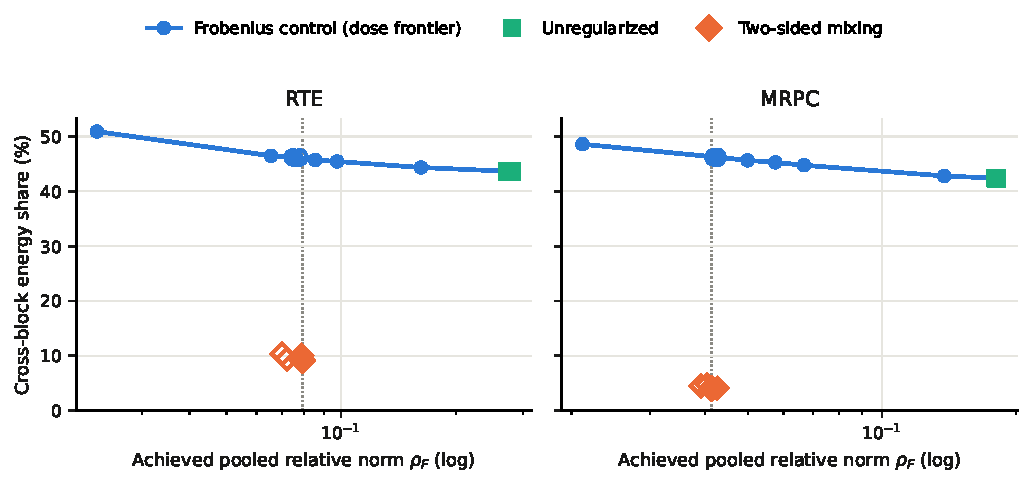
\includegraphics[width=\linewidth]{figures/focused_cross_vs_norm.pdf}
\caption{Cross-band energy share versus achieved update magnitude. The Frobenius control's full dose frontier (calibration seed; smaller markers) and the unregularized endpoint lie on one flat curve on both tasks; mixing-regularized runs (diamonds; open markers are the three confirmation seeds) sit far below at the same achieved magnitude (dotted line: the mixing arm's calibration norm). Calibration points are exploratory; confirmation points are the registered seed replicates.}
\label{fig:crossvsnorm}
\end{figure}

% BEGIN GENERATED FOCUSED CONFIRMATION
% Generated by scripts/build_focused_tables.py from data/focused_norm/runs.csv.
\begin{table}[t]
\centering
\caption{Confirmation of the matched-magnitude contrast across seeds 42, 17, and 123
(mean$\pm$sample SD, $n=3$), fixed-step endpoints, common protocol of
Section~\ref{sec:matchedcontrol}. Cross, LL, and TT are pooled energy percentages;
the probe is masked-token cross-entropy under the frozen original MLM head;
accuracy is the inner-selection split at the fixed step, scaled by 100. The norm-control
row states the per-seed achieved matching errors
$e_s=|\rho_{\mathrm{NORM},s}/\rho_{\mathrm{MIX},s}-1|$ against the declared
$\pm5\%$ rule; matching status is measured on these runs, not inherited from calibration.}
\label{tab:matchedconfirmation}
\begin{adjustbox}{max width=\linewidth}
\begin{tabular}{llcccccc}
\toprule
Task & Condition & $\rho_F$ & Cross (\%) & LL (\%) & TT (\%) & Probe CE & Acc \\
\midrule
RTE & Unregularized & $0.2751 \pm 0.0041$ & $43.7 \pm 0.0$ & $45.9 \pm 0.1$ & $10.4 \pm 0.0$ & $2.89 \pm 0.17$ & $72.4 \pm 0.6$ \\
RTE & Two-sided mixing & $0.0736 \pm 0.0046$ & $10.0 \pm 0.5$ & $45.2 \pm 0.9$ & $44.8 \pm 1.4$ & $2.94 \pm 0.29$ & $72.6 \pm 3.1$ \\
RTE & Norm control ($\beta=7.5$; match errors 8.0, 5.2, 7.5\%) & $0.0759 \pm 0.0016$ & $46.2 \pm 0.0$ & $40.7 \pm 0.0$ & $13.1 \pm 0.0$ & $2.61 \pm 0.08$ & $74.6 \pm 0.5$ \\
\midrule
MRPC & Unregularized & $0.1802 \pm 0.0009$ & $42.4 \pm 0.1$ & $48.0 \pm 0.1$ & $9.6 \pm 0.1$ & $2.75 \pm 0.07$ & $84.9 \pm 0.2$ \\
MRPC & Two-sided mixing & $0.0407 \pm 0.0017$ & $4.5 \pm 0.3$ & $69.8 \pm 1.1$ & $25.8 \pm 1.4$ & $2.84 \pm 0.17$ & $84.5 \pm 0.5$ \\
MRPC & Norm control ($\beta=27$; match errors 5.5, 6.7, 0.1\%) & $0.0423 \pm 0.0005$ & $46.2 \pm 0.1$ & $40.6 \pm 0.2$ & $13.2 \pm 0.1$ & $2.57 \pm 0.11$ & $84.8 \pm 0.2$ \\
\bottomrule
\end{tabular}
\end{adjustbox}
\end{table}
% END GENERATED FOCUSED CONFIRMATION

Table~\ref{tab:matchedconfirmation} and Figure~\ref{fig:crossvsnorm} give the confirmed result. At overlapping update magnitudes (per-seed matching errors $0.1$--$8.0\%$; three of six paired seeds marginally exceed the calibration tolerance, an observed seed-level norm variability we report rather than re-tune), the Frobenius control leaves the cross-band share at or slightly above the unregularized level ($46.2\%$ versus $42$--$44\%$), while the mixing penalty reduces it to $10.0\pm0.5\%$ (RTE) and $4.5\pm0.3\%$ (MRPC). In absolute terms the mixing arm carries roughly $5\times$ (RTE) and $11\times$ (MRPC) less cross-band energy than the matched control, and $60\times$/$185\times$ less than unregularized adaptation. Across the entire dose frontier, spanning pooled norms from $0.36$ to $0.02$, the control's cross share stays within $43$--$51\%$ and drifts mildly \emph{upward} at extreme shrinkage---the opposite direction of the mixing effect. Within this tested family, magnitude control does not reproduce the suppression; the geometric effect is attributable to the pretrained-frame penalty, though universal spectral specificity would require the deferred frame and scaler controls.

The surviving update occupies different bands on different tasks: on RTE the mixing arm is nearly block-diagonal ($45.2\pm0.9\%$ leading, $44.8\pm1.4\%$ tail), while on MRPC it is leading-dominated ($69.8\pm1.1\%$), and the insertion offset accounts for almost none of this (learned-since-insertion decompositions differ by under five points). Fixed-endpoint task accuracies are statistically indistinguishable across arms on both tasks (RTE $72.4/72.6/74.6\pm0.5$--$3.1$; MRPC $84.9/84.5/84.8\pm0.2$--$0.5$), and every run passes an explicit learning-health check. The frozen-original-head probe is a secondary functional measurement: all trained arms sit $0.5$--$0.9$ nats above the genuine unadapted reference ($2.10$), and the mixing arm is not closer to it than the matched control---geometric confinement does not by itself track pretrained-behavior proximity.

\subsection{Which blocks change under mixing control?}
The aggregate off-tail ratio combines direct leading adaptation and cross interaction. To separate them, we reconstruct the four energy fractions from the saved per-matrix diagnostics, square before averaging, and retain equal weighting of modules within each run. Figure~\ref{fig:allocation} shows the resulting leading, cross, and tail allocation. Appendix~\ref{app:blockallocation} gives all four blocks and accounts for the small finite-precision difference between the recorded coordinate and ambient norms.

\begin{figure}[t]
\centering
% BEGIN GENERATED BLOCK FIGURE
\begin{minipage}[t]{0.19\linewidth}
\centering\small RTE ($n=2$)\par\smallskip
\allocationbar{A}{0.4638846}{0.4340701}{0.1020454}\par\smallskip
\allocationbar{B}{0.4363037}{0.4355409}{0.1281555}\par\smallskip
\allocationbar{C}{0.4430157}{0.2745369}{0.2824474}\par\smallskip
\allocationbar{N}{0.4444444}{0.4444444}{0.1111112}\par\smallskip
\end{minipage}
\hfill
\begin{minipage}[t]{0.19\linewidth}
\centering\small MRPC ($n=2$)\par\smallskip
\allocationbar{A}{0.4656407}{0.4324835}{0.1018758}\par\smallskip
\allocationbar{B}{0.4962905}{0.4031637}{0.1005458}\par\smallskip
\allocationbar{C}{0.6364850}{0.1008374}{0.2626776}\par\smallskip
\allocationbar{N}{0.4444444}{0.4444444}{0.1111112}\par\smallskip
\end{minipage}
\hfill
\begin{minipage}[t]{0.19\linewidth}
\centering\small CoLA ($n=2$)\par\smallskip
\allocationbar{A}{0.4574255}{0.4374997}{0.1050748}\par\smallskip
\allocationbar{B}{0.4561447}{0.4238463}{0.1200090}\par\smallskip
\allocationbar{C}{0.5698152}{0.2108519}{0.2193329}\par\smallskip
\allocationbar{N}{0.4444444}{0.4444444}{0.1111112}\par\smallskip
\end{minipage}
\hfill
\begin{minipage}[t]{0.19\linewidth}
\centering\small STS-B ($n=2$)\par\smallskip
\allocationbar{A}{0.4625905}{0.4346104}{0.1027991}\par\smallskip
\allocationbar{B}{0.4634592}{0.4196426}{0.1168983}\par\smallskip
\allocationbar{C}{0.5226626}{0.1371491}{0.3401883}\par\smallskip
\allocationbar{N}{0.4444444}{0.4444444}{0.1111112}\par\smallskip
\end{minipage}
\hfill
\begin{minipage}[t]{0.19\linewidth}
\centering\small SST-2 ($n=1$)\par\smallskip
\allocationbar{A}{0.4651930}{0.4333157}{0.1014913}\par\smallskip
\allocationbar{B}{0.4875879}{0.4019357}{0.1104764}\par\smallskip
\allocationbar{C}{0.5573737}{0.1720633}{0.2705630}\par\smallskip
\allocationbar{N}{0.4444444}{0.4444444}{0.1111112}\par\smallskip
\end{minipage}
% END GENERATED BLOCK FIGURE
\par\smallskip
{\small\textcolor{black!80}{\rule{1em}{1ex}} Leading--leading\quad
\textcolor{black!45}{\rule{1em}{1ex}} Cross\quad
\textcolor{black!15}{\rule{1em}{1ex}} Tail--tail}
\caption{Leading/cross/tail allocation, averaged over modules then $n$ seeds. A: no penalty; B: left-only; C: two-sided. N is the dimension-only reference $(4/9,4/9,1/9)$, not a training run. C reduces cross share but retains a leading block; Table~\ref{tab:mixingmain} supplies magnitude and dispersion, and Appendix~\ref{app:blockallocation} supplies each seed's four fractions.}
\label{fig:allocation}
\end{figure}

Without regularization, cross blocks contain approximately 43\% of update energy, the leading block 46\%, and the tail 10\%. Under C, cross share is 10--27\%, tail share 22--34\%, and leading share 44--64\%; the last rises in four task means. This is consistent with Proposition~\ref{prop:mixing}, which permits a leading modification after cross decoupling. It is not evidence that this modification is task-specific: constant scalers leave an identity-shaped leading core, and the measured delta includes initialization. Appendix~\ref{app:offset} quantifies the prescribed initial contribution. A larger fraction also need not mean larger absolute energy.

Run means conceal module heterogeneity (Appendix~\ref{app:blockallocation}); they do not show that every layer's leading subspace is stabilized.

\subsection{One-sided control and factor asymmetry}
B has the highest mean score on RTE, MRPC, and CoLA while its cross shares remain approximately 40--44\% (Table~\ref{tab:mixingmain}). Better task scores therefore do not coincide with stronger cross suppression across these conditions. The variation is too sparsely replicated to identify a benefit or its cause. In all nine A/B pairs, $\mu_E$ falls while $\nu_D$ rises; the reciprocal factor symmetry in Section~\ref{sec:mixing} shows why this alone cannot demonstrate transfer of learning to the unpenalized side. Optimization and generic regularization remain alternative explanations.

\paragraph{Interpreting normalized geometry.}
The changed norm ratios exclude an explanation based only on multiplying the \emph{same trained matrix} by a scalar. They do not exclude the possibility that magnitude-only regularization during training would produce similar geometry. The distinction is between an observed change in normalized placement and a magnitude-independent benefit, which requires a norm-matched training control. These selected endpoints also concern update geometry, not the time at which mixing arises during learning.

An isotropically oriented perturbation has expected leading/cross/tail fractions $k^2/d^2$, $2kr/d^2$, and $r^2/d^2$ (Appendix~\ref{app:dimension}). Figure~\ref{fig:allocation} makes this dimension-only reference explicit. A lies nearby, but agreement of three aggregate fractions is not a test of isotropy or evidence that pretrained structure is unused. Equal-dimensional random-frame controls and measurements of other adapters are needed to distinguish those interpretations.

\subsection{Downstream viability of the instruments}
Table~\ref{tab:glue_results_base_large} retains the six-task GLUE subset on both RoBERTa backbones as evidence of task learning. Comparing the spectral rows, the rotated core has a higher average on base and a lower average on large: rotations are not uniformly better. Proposition~\ref{prop:approximation} concerns available directions, not guaranteed performance gains. The mixing intervention itself disables rotations.

\begin{table}[t]
\centering
\caption{Reported RoBERTa results on a six-task GLUE subset, mean$\pm$SD, multiplied by 100. Imported reference runs~\citep{albert2025randlora} and spectral runs use different tuning protocols and are grouped separately; this is not a matched ranking. MRPC is accuracy throughout. Avg6 is the mean of the six displayed metrics, not a full GLUE score; MNLI and QQP are absent.}
\label{tab:glue_results_base_large}
\begin{adjustbox}{max width=\linewidth}
\begin{tabular}{@{}lccccccc@{}}
\toprule
Method & SST-2 & MRPC Acc. & CoLA & QNLI & RTE & STS-B & Avg6 \\
\midrule
% BEGIN GENERATED GLUE ROWS
\multicolumn{8}{c}{RoBERTa-base} \\
\midrule
\multicolumn{8}{l}{\textit{Imported reference runs (RandLoRA protocol; five runs)}} \\
VeRA-1024 & 91.9{\scriptsize$\pm$0.4} & 88.4{\scriptsize$\pm$1.2} & 59.9{\scriptsize$\pm$2.2} & 90.5{\scriptsize$\pm$0.4} & 74.9{\scriptsize$\pm$1.5} & 90.4{\scriptsize$\pm$0.2} & 82.67 \\
LoRA-4 & 94.4{\scriptsize$\pm$0.5} & 87.3{\scriptsize$\pm$0.2} & 58.4{\scriptsize$\pm$0.8} & 92.7{\scriptsize$\pm$0.2} & 71.5{\scriptsize$\pm$1.2} & 90.5{\scriptsize$\pm$0.1} & 82.47 \\
RandLoRA-64 & 92.2{\scriptsize$\pm$0.3} & 88.0{\scriptsize$\pm$1.5} & 59.4{\scriptsize$\pm$2.1} & 91.3{\scriptsize$\pm$0.4} & 74.7{\scriptsize$\pm$1.9} & 90.3{\scriptsize$\pm$0.2} & 82.65 \\
\addlinespace
\multicolumn{8}{l}{\textit{Spectral instruments (reported protocol; six seeds)}} \\
UIOrthoLoRA & 94.8{\scriptsize$\pm$0.3} & 92.0{\scriptsize$\pm$1.0} & 64.4{\scriptsize$\pm$1.0} & 92.4{\scriptsize$\pm$0.1} & 78.7{\scriptsize$\pm$1.0} & 90.7{\scriptsize$\pm$0.1} & 85.50 \\
UILinLoRA & 93.1{\scriptsize$\pm$1.0} & 90.0{\scriptsize$\pm$1.0} & 65.8{\scriptsize$\pm$1.0} & 92.4{\scriptsize$\pm$0.2} & 76.2{\scriptsize$\pm$1.0} & 90.6{\scriptsize$\pm$0.1} & 84.68 \\
\midrule
\multicolumn{8}{c}{RoBERTa-large} \\
\midrule
\multicolumn{8}{l}{\textit{Imported reference runs (RandLoRA protocol; five runs)}} \\
VeRA-256 & 95.8{\scriptsize$\pm$0.3} & 89.3{\scriptsize$\pm$1.2} & 65.3{\scriptsize$\pm$1.1} & 94.1{\scriptsize$\pm$0.3} & 81.6{\scriptsize$\pm$0.8} & 91.8{\scriptsize$\pm$0.1} & 86.32 \\
LoRA-4 & 95.5{\scriptsize$\pm$0.2} & 87.2{\scriptsize$\pm$0.7} & 64.7{\scriptsize$\pm$1.2} & 94.5{\scriptsize$\pm$0.1} & 83.6{\scriptsize$\pm$0.4} & 91.8{\scriptsize$\pm$0.1} & 86.22 \\
RandLoRA-100 & 95.5{\scriptsize$\pm$0.3} & 90.1{\scriptsize$\pm$0.4} & 67.4{\scriptsize$\pm$0.3} & 94.1{\scriptsize$\pm$0.3} & 84.5{\scriptsize$\pm$0.3} & 91.4{\scriptsize$\pm$0.6} & 87.17 \\
\addlinespace
\multicolumn{8}{l}{\textit{Spectral instruments (reported protocol; six seeds)}} \\
UIOrthoLoRA & 96.3{\scriptsize$\pm$0.3} & 92.5{\scriptsize$\pm$0.2} & 67.4{\scriptsize$\pm$0.5} & 95.0{\scriptsize$\pm$0.1} & 86.0{\scriptsize$\pm$0.2} & 92.1{\scriptsize$\pm$0.2} & 88.22 \\
UILinLoRA & 96.3{\scriptsize$\pm$0.2} & 93.4{\scriptsize$\pm$0.7} & 68.7{\scriptsize$\pm$1.0} & 94.7{\scriptsize$\pm$0.1} & 86.0{\scriptsize$\pm$1.1} & 92.0{\scriptsize$\pm$0.2} & 88.52 \\
% END GENERATED GLUE ROWS
\bottomrule
\end{tabular}
\end{adjustbox}
\end{table}

The imported LoRA and VeRA rows are RandLoRA's reference runs, not the original methods' canonical results. Different ranks, schedules, seed aggregation, and intermediate-task initialization can materially change such comparisons~\citep{hu2022lora,kopiczko2023vera}. The table preserves the reported observations without treating their cross-protocol gaps as method effects. Appendix~\ref{app:cost} gives configuration-derived costs separately from historical parameter counts that require run-level reconciliation.

GPT-2 Medium generation provides additional task-learning evidence (Appendix~\ref{app:generation}), but no matched spectral measurements. Functional retention requires a separate, matched evaluation (Appendix~\ref{app:retention}).

\paragraph{Computational scope.}
The unrotated $d=768,r=256$ instrument trains 1,792 entries per matrix but stores 1,179,648 frozen basis entries: 56.6M across 48 matrices, or 113.2 MB at two bytes per entry. Two full-basis products cost approximately $2d^2$ multiply--accumulates per token, versus $2d\ell$ for rank-$\ell$ LoRA, excluding regularization and backward computation. These are arithmetic counts, not measured speed ratios. Merging removes the inference branch. Appendix~\ref{app:cost} gives full accounting, and Appendix~\ref{app:loggedcost} reports the available runtime/memory logs without inferring matched throughput.
\section{Related work}
\label{sec:related}

\paragraph{Efficient parameterizations.}
LoRA restricts update rank~\citep{hu2022lora}; AdaLoRA allocates an update's singular-value budget, not a fixed pretrained SVD~\citep{zhang2023adalora}. VeRA and RandLoRA learn scales around random factors, while DoRA and FourierFT use weight decomposition and Fourier coefficients~\citep{kopiczko2023vera,albert2025randlora,liu2024dora,gao2024parameter}. Intrinsic-dimension studies establish the usefulness of restricted parameter spaces~\citep{li2018measuring,aghajanyan2020intrinsic}; their dimension alone does not determine spectral placement.

\paragraph{Pretrained spectral information.}
SVDiff and SVFT precede fixed-basis coefficient tuning~\citep{han2023svdiff,lingam2024svft}. PiSSA and MiLoRA initialize free factors from leading and minor components, respectively~\citep{meng2024pissa,wang2025milora}; initialization is not continued confinement. KaSA combines a truncated pretrained component with singular-value-aware adaptation~\citep{wang2025kasa}. LoRA-XS and CorDA provide further decomposition-guided choices~\citep{balazy2024lora,yang2024corda}. Our focus is the constraint each choice imposes, not novelty of the SVD frame.

\paragraph{Rotations and scalers.}
Spectral Adapter's rotational form replaces a leading core by $R_U\Sigma_LR_V^\top$, giving $C_{LL}=R_U\Sigma_LR_V^\top-\Sigma_L$ and zero other blocks~\citep{zhang2024spectral}. Our tail instrument instead adds a trainable core to the frozen pretrained tail. PSOFT acts in a principal subspace with compact orthogonal transforms and vector relaxations~\citep{wu2026psoft}; these are important antecedents, not identical update forms. OFT and BOFT provide ambient orthogonal transforms~\citep{qiu2023oft,liu2024boft}. SSF and $(\mathrm{IA})^3$ learn feature scales~\citep{lian2022ssf,liu2022ia3}, while DoRA separates weight magnitude and direction. Diagonal scaling has these precedents; our commutator identity characterizes a scaler relative to a fixed projector, not every component of those methods.

\paragraph{Orthonormality versus confinement.}
SORSA trains principal singular factors, freezes a residual, and penalizes deviations of the factors' Gram matrices from identity~\citep{cao2025sorsa}. Our rotations preserve prescribed spans; our scaler penalty acts on fixed-projector overlaps. Orthonormal factors can span a different subspace, so these constraints are distinct. This is an analytical contrast, not a measured advantage over SORSA.

\paragraph{Geometry, intervention, and retention.}
\citet{shuttleworth2025illusion} compare LoRA and full-fine-tuning spectra and intervene on intruder directions; \citet{xie2026intruder} additionally studies spectral thresholds and norm-matched interventions. Those interventions do not supply our missing within-family controls. CLoRA regularizes subspaces~\citep{lu2025controlled}; \citet{biderman2024lora} study adaptation and forgetting. We focus on ambient scaling around spectral cores, distinguishing factor-level constraints from effective-update measurements and behavioral outcomes.
\section{Discussion and limitations}
\label{sec:discussion}

\paragraph{Reading spectral evidence.}
A spectral report should declare the pretrained checkpoint and cutoff rule; separate total and since-insertion deltas; report all block energies and their dimension-only reference; and pair norm and subspace diagnostics with task outcomes on the same checkpoint. The cutoff here is determined by the 256-direction adaptation span, not selected for a large spectral gap. A reusable metric specification, including non-maximal-angle drift and initialization checks, appears in Appendix~\ref{app:reportcard}. This prevents one ``preservation'' score from conflating reduced interaction, residual leading modification, and update shrinkage.

\paragraph{What the tail reference does and does not imply.}
Our projection identities require no task-alignment assumption, but do not establish the tail's empirical suitability. That requires equal-dimensional leading, tail, and mixed/random controls. Increased within-tail expressivity likewise need not improve a trained model: useful directions, optimization, and the statistical cost of added capacity all matter.

\paragraph{Scope of the intervention.}
The five-task intervention has limited replication, a single penalty strength, and validation-selected endpoints at unequal steps. Norm-matched, centered-scaler, random-projector, and head-only controls are absent. The data therefore cannot separate spectral specificity from shrinkage, homogenization, or head-dominated learning. Nor do the archived ratios determine the initialization-corrected block energies or identity alignment of the leading core. Our approximation identities concern representability; the mixing bounds require attained factor norms, and ranked stability additionally requires spectral separation.

\paragraph{External validity and comparison coverage.}
The block measurements use one backbone and one adapter family. Although the coordinates apply algebraically to LoRA, full fine-tuning, and spectral alternatives, the present data do not demonstrate cross-method geometric differences. The supporting benchmarks are not uniformly tuned comparisons. Testing the same controls and behavior probes on a generative backbone is necessary before extending the findings beyond this setting.

\section{Conclusion}
\label{sec:conclusion}
Spectral confinement, cross-block decoupling, and ranked-subspace stability are distinct. Tail rotations change within-span capacity; ambient scalers can break confinement, and suppressing their mixing leaves a leading contribution when the core contains one. The archived intervention exhibits that distinction alongside substantial shrinkage, without isolating spectral specificity. A defensible account of adaptation must separate its reference frame, insertion offset, effective magnitude, and block allocation. This is the role of the spectral instruments, independently of which adapter scores highest.
\clearpage
\section*{Reproducibility statement}
Complete proofs appear in Appendix~\ref{app:proofs}, training and metric definitions in Appendix~\ref{app:details}, and computational costs in Appendix~\ref{app:cost}. Equation~\eqref{eq:unified} specifies the practical parameterization separately from the tail-only reference. Archived summary and module-level records, with analysis scripts, reproduce the mixing tables and block-allocation figure; a separate synthetic-matrix script checks the algebraic identities and boundary cases. These checks do not rerun model training. Supporting benchmark tables distinguish imported comparisons from the spectral-variant results.

\begin{samepage}
\section*{AI use statement}
Generative AI tools were used to assist with restructuring and drafting the manuscript, literature lookup, mathematical formulation and proof drafting, interpretation of existing experimental records, and design of additional experiments. AI assistance was also used to write scripts for consistency checks and table reconstruction. The numerical experimental results reported here come from existing research records, not generated or simulated outcomes attributed to unperformed training runs.
\par\end{samepage}

\begin{samepage}
\section*{Ethics statement}
The study analyzes adaptation of existing language models using existing benchmarks. Weight-space stability does not certify factual correctness, fairness, privacy, or safe behavior. Efficient adaptation can reduce training costs but can also facilitate harmful specialization or preserve biases present in a base model. Our structural claims should not be interpreted as deployment guarantees.\par
\end{samepage}
\bibliography{reference}
\bibliographystyle{iclr2027_conference}
\clearpage
\appendix
\section{Proofs and boundary cases}
\label{app:proofs}

\subsection{Fixed coefficients and within-tail flexibility}
\label{app:approximation}
Let $\widehat G=U^\top G V$ and partition it into the four coordinate blocks. Orthogonal invariance gives
\begin{equation}
\fro{G-U_T H V_T^\top}^2
=\fro{\widehat G_{LL}}^2+\fro{\widehat G_{LT}}^2
+\fro{\widehat G_{TL}}^2+\fro{\widehat G_{TT}-H}^2.
\end{equation}
For a free core the last term is minimized at $H=\widehat G_{TT}$. For a diagonal core it is minimized by $h_i=(\widehat G_{TT})_{ii}$, leaving the off-diagonal entries unchanged. Substitution proves Proposition~\ref{prop:approximation}. An SVD of the minimizing free core gives the representation~\eqref{eq:rotations}; this is an existence statement, not a guarantee for a particular optimizer or partial-rotation block.

If the free core is additionally constrained to rank at most $q\le r$, applying truncated SVD to $\widehat G_{TT}$ gives minimum squared error
\begin{equation}
\fro{G}^2-\sum_{j=1}^q\sigma_j(\widehat G_{TT})^2.
\end{equation}
This expression keeps the outside-tail residual explicit. It should not be replaced by the best unrestricted rank-$q$ approximation error of the entire $G$, whose singular directions may lie outside the selected tail.

\subsection{Proof of the unified mixing bounds}
\label{app:mixingproof}
Because $U,V$ are orthogonal,
\begin{equation}
C=A\begin{bmatrix}S_L&0\\0&H\end{bmatrix}B.
\end{equation}
Direct multiplication gives
\begin{align}
C_{LL}&=A_{LL}S_LB_{LL}+A_{LT}HB_{TL},\\
C_{LT}&=A_{LL}S_LB_{LT}+A_{LT}HB_{TT},\\
C_{TL}&=A_{TL}S_LB_{LL}+A_{TT}HB_{TL},\\
C_{TT}&=A_{TL}S_LB_{LT}+A_{TT}HB_{TT}.
\end{align}
Symmetry yields $\op{A_{TL}}=\op{A_{LT}}=\mu$ and $\op{B_{TL}}=\op{B_{LT}}=\nu$. Orthogonal compression bounds the diagonal blocks of $A$ by $e$ and those of $B$ by $d_s$. Apply the triangle inequality and submultiplicativity to each product to obtain~\eqref{eq:blockbound1}--\eqref{eq:blockbound2}.

For the tail-only core, $s=0$ and
\begin{equation}
C-C_{\mathrm{tail}}=\begin{bmatrix}C_{LL}&C_{LT}\\C_{TL}&0\end{bmatrix}.
\end{equation}
For any block vector $(x,y)$, the norms of the two output blocks are bounded componentwise by
\begin{equation}
\begin{bmatrix}\op{C_{LL}}&\op{C_{LT}}\\\op{C_{TL}}&0\end{bmatrix}
\begin{bmatrix}\|x\|_2\\\|y\|_2\end{bmatrix}.
\end{equation}
Taking a supremum and bounding the norm of this nonnegative $2\times2$ matrix by its Frobenius norm proves
\begin{equation}
\op{C-C_{\mathrm{tail}}}
\le\sqrt{\op{C_{LL}}^2+\op{C_{LT}}^2+\op{C_{TL}}^2}.
\end{equation}
Substitution gives~\eqref{eq:offbound}. If the stated factor norms remain bounded, its right-hand side goes to zero as $\mu,\nu\to0$.

For the general core, let $C_{\mathrm{diag}}=\diag(C_{LL},C_{TT})$. The off-diagonal block matrix satisfies the exact identity
\begin{equation}
\op{C-C_{\mathrm{diag}}}=\max\{\op{C_{LT}},\op{C_{TL}}\}.
\end{equation}
The cross-block bounds therefore imply convergence to the set of block-diagonal updates when $e,d_s,h_s,s$ are bounded and $\mu,\nu\to0$. The term $A_{LL}S_LB_{LL}$ need not vanish. This proves Corollary~\ref{cor:confinement} and states precisely the different limits in the two cases.

\subsection{Confinement does not prevent singular-value crossings}
\label{app:crossing}
For a tail-only update without ambient scaling,
\begin{equation}
U^\top(W_0+\Delta)V=
\begin{bmatrix}\Sigma_L&0\\0&\Sigma_T+H\end{bmatrix}.
\end{equation}
The singular values are the union of those of the two diagonal blocks, which proves the sufficient condition~\eqref{eq:nocrossing}. Consider $W_0=\diag(2,1)$, cutoff $k=1$, and $\Delta=\diag(0,2)$. The update is strictly tail-supported with no cross mixing and no leading-block modification, but $W_0+\Delta=\diag(2,3)$ has the other coordinate as its top singular direction. Its largest-principal-angle sine relative to the original leading direction is one. Thus block decoupling and stability of the top-ranked subspace are distinct even in a two-dimensional example.

\subsection{Rectangular weights and complete energy accounting}
\label{app:rectangular}
For $W_0\in\mathbb R^{m\times n}$, select $k\le\min(m,n)$ leading singular vectors and define
\begin{equation}
P_L=U_LU_L^\top,\quad P_T=I_m-P_L,\qquad
Q_L=V_LV_L^\top,\quad Q_T=I_n-Q_L.
\end{equation}
Then $\Delta_{ab}=P_a\Delta Q_b$ gives
\begin{equation}
\Delta=\sum_{a,b}\Delta_{ab},\qquad
\fro{\Delta}^2=\sum_{a,b}\fro{\Delta_{ab}}^2.
\end{equation}
Pairwise Frobenius inner products vanish because complementary projectors multiply to zero. The tail here is the full complement and includes any unmatched null directions. A chosen adapter may span only a subset of it; that available subspace must not be confused with the diagnostic complement. Complete orthogonal bases recover the corresponding coordinate blocks. The square attention-matrix experiment avoids this issue, but an economy-SVD diagnostic is not automatically exhaustive for other layers.

\subsection{A dimension-only reference for allocation}
\label{app:dimension}
Let the vectorized nonzero update have a rotationally invariant direction in the $d^2$-dimensional matrix space. By symmetry each squared coordinate has expected fraction $1/d^2$ of the total. The leading, cross, and tail blocks have $k^2$, $2kr$, and $r^2$ coordinates, respectively. Their expected energy fractions are therefore $k^2/d^2$, $2kr/d^2$, and $r^2/d^2$. For $r/d=1/3$, these are $4/9$, $4/9$, and $1/9$, with off-tail expectation $8/9$. The square root $\sqrt{8/9}\simeq0.9428$ is a reference on the norm-ratio scale, not the expectation $\mathbb E[q_{\off}]$. These calculations are a null reference, not a fitted model or a statistical test of the observed updates.

\subsection{The scaler penalty as a projector commutator}
\label{app:commutator}
In the complete $U$ basis, $P$ is $\diag(I_k,0)$. Writing $A=U^\top EU$ gives
\begin{equation}
U^\top(EP-PE)U=
\begin{bmatrix}0&-A_{LT}\\A_{TL}&0\end{bmatrix}.
\end{equation}
Because $A$ is symmetric, orthogonal invariance yields $\|EP-PE\|_F^2=2\|A_{LT}\|_F^2$. In ambient coordinates, the $(i,j)$ entry of the commutator is $(\epsilon_i-\epsilon_j)P_{ij}$. Squaring and combining its symmetric pairs proves~\eqref{eq:commutator}. Equivalently, the penalty is $\epsilon^\top L_P\epsilon$, where $L_P$ is the graph Laplacian with off-diagonal edge weights $P_{ij}^2$. Every summand is nonnegative. Zero penalty therefore means equal scales across every nonzero edge, or constant scales on each connected component. A connected graph has only globally constant scales in this nullspace. A disconnected projector permits different constants on disconnected components; for a coordinate-aligned projector, all off-diagonal weights vanish and every ambient diagonal scaler commutes with it. The result is conditional on the fixed pretrained projector, not a measured connectivity claim for the experiment.

\subsection{Random-projector reference and scaler homogenization}
\label{app:randompenalty}
Write $J_P(\epsilon)=\epsilon^\top L_P\epsilon$ for~\eqref{eq:commutator}. Since $L_P\mathbf1=0$, adding a constant to every scale does not change the penalty. Under the penalty alone, $\dot\epsilon=-2\lambda L_P\epsilon$ preserves $\bar\epsilon$ and damps each positive-eigenvalue component of $L_P$. On a connected graph it converges to $\bar\epsilon\mathbf1$. This statement concerns ordinary gradient flow of this isolated quadratic, not AdamW with a task loss; neither shrinkage of the mean nor convergence of the trained model follows from it.

For a uniformly random rank-$k$ orthogonal projector $P$ in $\mathbb R^d$, and a fixed scaler vector independent of $P$,
\begin{equation}
\mathbb E_P[J_P(\epsilon)]
=\frac{k(d-k)}{(d-1)(d+2)}\|\epsilon-\bar\epsilon\mathbf1\|_2^2.
\label{eq:randompenalty}
\end{equation}
To verify the constant, write $P=QQ^\top$ for the first $k$ columns of a Haar orthogonal matrix. The spherical fourth moments give $\mathbb E[P_{ii}^2]=k(k+2)/(d(d+2))$. Since $\sum_{ij}P_{ij}^2=k$, symmetry gives $\mathbb E[P_{ij}^2]=k(d-k)/(d(d-1)(d+2))$ for $i\ne j$. Substitute into~\eqref{eq:commutator} and use $\sum_{i<j}(\epsilon_i-\epsilon_j)^2=d\|\epsilon-\bar\epsilon\mathbf1\|_2^2$.

This expectation motivates a centered-scaler control. It does not equate one fixed random projector with the pretrained projector: their positive-eigenvalue directions and strengths generally differ. It also cannot be substituted into training when the learned scalers depend on the sampled projector. A shared scalar nullspace alone does not imply identical trajectories or endpoints.

\subsection{Factor-scale identities}
Write the inner matrix in~\eqref{eq:unified} as $K$. For any $a>0$, $(aE)K(D/a)=EKD$. Because each mixing operator is linear in its respective scaler, this transformation multiplies its two magnitudes by $a$ and $1/a$. For $S_L=0$, the additional identity
\begin{equation}
(aE)U_T(H/a^2)V_T^\top(aD)=E U_T H V_T^\top D
\end{equation}
shrinks both squared Frobenius penalties by $a^2$. It can make a raw factor penalty arbitrarily small with a fixed effective update if the core is allowed to diverge. It does not refute the bounded-factor confinement statement, nor does it imply that the optimizer follows this path. It motivates measuring the actual update and the norms appearing in the bound.
\section{Experimental details}
\label{app:details}

\subsection{Backbones, tasks, and placement}
The broader language-understanding evaluation uses RoBERTa-base and RoBERTa-large on a six-task GLUE subset: CoLA, SST-2, MRPC, STS-B, QNLI, and RTE~\citep{wang2018glue}. The mixing intervention uses RoBERTa-base on five of these tasks, excluding QNLI. Neither evaluation covers MNLI or QQP. Table~\ref{tab:glue_results_base_large} reports Matthews correlation for CoLA, accuracy for SST-2/MRPC/QNLI/RTE, and Pearson correlation for STS-B, consistently across spectral and imported comparisons. The separate mixing intervention reports F1 for MRPC; its other task metrics are unchanged. Results use the official validation splits. Pretrained backbone parameters are frozen, and adapters and the prediction head train jointly. The adapted modules are the query, key, value, and attention-output projections; feed-forward projections remain frozen.

\subsection{Training configuration}
The training recipe uses AdamW with separate adapter and head learning rates, linear decay, a 6\% warmup fraction, batch size 64, and maximum sequence length 256. Table~\ref{tab:recipe} gives the task-specific settings recorded for RoBERTa-base. These task-specific configurations are not a common hyperparameter search across all methods in the supporting benchmark table.

\begin{table}[ht]
\centering
\caption{RoBERTa-base training settings from the experimental protocol. The scaler value initializes both ambient diagonal scalers.}
\label{tab:recipe}
\begin{tabular}{lccccc}
\toprule
Task & Epochs & Head LR & Adapter LR & Scaler & Coefficients\\
\midrule
CoLA & 80 & $5\cdot10^{-3}$ & $3\cdot10^{-2}$ & $10^{-2}$ & $10^{-1}$\\
SST-2 & 40 & $10^{-2}$ & $4\cdot10^{-2}$ & $10^{-1}$ & $10^{-1}$\\
MRPC & 30 & $10^{-3}$ & $5\cdot10^{-2}$ & $10^{-1}$ & $10^{-1}$\\
STS-B & 60 & $5\cdot10^{-3}$ & $10^{-2}$ & $10^{-1}$ & $10^{-1}$\\
QNLI & 25 & $10^{-3}$ & $2\cdot10^{-2}$ & $10^{-1}$ & $10^{-1}$\\
RTE & 90 & $5\cdot10^{-4}$ & $10^{-2}$ & $10^{-2}$ & $10^{-2}$\\
\bottomrule
\end{tabular}
\end{table}

Adapter dropout is zero and the nominal adapter scaling coefficient is one. The broad GLUE configurations use $k_{\mathrm{val}}=256$, with $k_{\mathrm{vec}}=0$ for UILinLoRA and 64 for UIOrthoLoRA. The mixing study uses 256 and zero, respectively. Compact rotations, when enabled, use an orthogonal parameterization; only the selected sub-block is rotated. With nonzero initialized scalers and coefficients, the practical adapter need not have zero initial delta. The measured displacement from $W_0$ includes that initial contribution.

\subsection{Initialization and residual leading structure}
\label{app:offset}
For the prescribed identity rotations, $E=D=s_0I$, $H=h_0I_r$, and $S_L=I_k$, insertion adds
\begin{equation}
\Delta_{\mathrm{init}}=s_0^2(U_LV_L^\top+h_0U_TV_T^\top),\quad
\fro{\Delta_{\mathrm{init}}}=s_0^2\sqrt{k+rh_0^2},\quad
p_{LL,\mathrm{init}}=\frac{k}{k+rh_0^2}.
\label{eq:initoffset}
\end{equation}
The cross blocks are initially zero. With $k=512,r=256$, the prescribed norm is approximately $0.22684$ for MRPC/STS-B/SST-2, $0.0022684$ for CoLA, and $0.0022628$ for RTE. Leading energy is approximately 99.50\% in the first four tasks and 99.995\% in RTE. These are analytical values from Table~\ref{tab:recipe}, not recovered checkpoint measurements. The missing pretrained matrix norms prevent inferring their relative contribution to the trained update from these values alone.

For an attained leading block, define its identity alignment
\begin{equation}
\eta_I=\frac{(\operatorname{tr}C_{LL})^2}{k\fro{C_{LL}}^2},\qquad
0\le\eta_I\le1\quad(C_{LL}\ne0).
\label{eq:identityalignment}
\end{equation}
It equals the fraction of leading-block Frobenius energy in the projection onto $\operatorname{span}(I_k)$. Under constant scalers and $S_L=I_k$, $C_{LL}=abI_k$ has $\eta_I=1$ when $ab\ne0$, even though cross mixing vanishes. This motivates reporting $C-C_{\mathrm{init}}$, $C_{LL}-(\operatorname{tr}C_{LL}/k)I_k$, and centered scaler norms alongside total block energies. Subtracting the initialization and subtracting a fitted identity component answer different questions; neither can be reconstructed by subtracting squared norms. The current summaries lack the signed blocks and scaler vectors needed for these trained measurements.

\subsection{Seeds and checkpoint selection}
The broader spectral evaluation protocol reports six seeds $\{42,123,2021,17,31415,1054\}$; Table~\ref{tab:glue_results_base_large} retains its reported means and across-seed standard deviations. The imported comparison uses five runs. The mixing analysis uses the nine task/seed pairs with archived paired summary and module-level records: seeds 42 and 17 for RTE, MRPC, CoLA, and STS-B, and 42 for SST-2. These records permit independent reaggregation of the intervention, whereas the broad GLUE table is a report of the original evaluation, not a newly reconstructed six-seed experiment.

The ablation runner selects the best validation checkpoint using the same task metric subsequently reported, then reloads it for scoring and spectral measurements. Thus these validation scores are selection-conditioned, not untouched test estimates. Table~\ref{tab:mixingfull} reports each selected step; RTE seed-42 A/B/C select steps 312, 3198, and 1755. We report sample SD in the main table and every available seed in the appendix. With one or two seeds per task, these do not support precise confidence intervals or cross-task independence assumptions. Stepwise loss logs are not substituted for missing spectral trajectories.

\subsection{Metric definitions and aggregation}
For each adapted matrix, the reported metrics are
\begin{align}
\rho_F&=\fro{\Delta}/\fro{W_0},&
q_{\off}&=\fro{C_{\off}}/\fro{C},\\
\mathrm{Leak}_{LL}&=\op{C_{LL}}/\op{\Delta},&
C_{\off}&=\begin{bmatrix}C_{LL}&C_{LT}\\C_{TL}&0\end{bmatrix}.
\end{align}
The mixing magnitudes are operator norms, while their training penalties use squared Frobenius norms. Leading left and right drift use the largest-principal-angle sine between the leading subspaces of $W_0$ and $W_0+\Delta$. The tables average each metric across the 48 adapted modules within a run, then across available seeds. They do not pool module energies before normalization. Because each model is a single trained replicate, 48 modules do not constitute 48 independent experimental seeds.

\subsection{Complete mixing results}
\label{app:mixingtable}
The accompanying \texttt{scripts/build\_mixing\_tables.py} generates Tables~\ref{tab:mixingmain} and~\ref{tab:mixingfull} from the included per-task/seed CSV summaries. These records retain checkpoint steps and metric columns. The analysis includes the paired A/B/C runs and excludes separate smoke tests and C-only reruns. This makes the aggregation independently checkable without rerunning training.
\begin{table}[ht]
\centering
\caption{Every archived mixing run and its validation-selected step. A: no penalty; B: left-only; C: two-sided. Scores are in native metric units (MRPC F1). Spectral values are means over 48 modules of that run: $\mu_E,\nu_D$ and drift use operator norms, while $\rho_F,q_{\off}$ are Frobenius norm ratios. Drift is the largest-angle sine, often near its ceiling.}
\label{tab:mixingfull}
\begin{adjustbox}{max width=\linewidth}
\begin{tabular}{llccccccccc}
\toprule
Task & Cond. & Seed & Step & Score & $\mu_E$ & $\nu_D$ & $\rho_F$ & $q_{\off}$ & Drift$_U$ & Drift$_V$\\
\midrule
% BEGIN GENERATED MIXING FULL
% Generated by scripts/build_mixing_tables.py from data/legacy_mixing/*.csv.
RTE & A & 17 & 6318 & 0.7798 & 1.392 & 1.464 & 0.389 & 0.948 & 1.000 & 1.000 \\
RTE & A & 42 & 312 & 0.7617 & 1.376 & 1.420 & 0.369 & 0.947 & 1.000 & 1.000 \\
RTE & B & 17 & 3510 & 0.7978 & 0.331 & 2.173 & 0.300 & 0.934 & 0.999 & 0.999 \\
RTE & B & 42 & 3198 & 0.7834 & 0.225 & 2.051 & 0.270 & 0.933 & 1.000 & 1.000 \\
RTE & C & 17 & 3588 & 0.7726 & 0.208 & 0.201 & 0.062 & 0.823 & 0.534 & 0.523 \\
RTE & C & 42 & 1755 & 0.7617 & 0.234 & 0.207 & 0.063 & 0.853 & 0.511 & 0.500 \\
\midrule
MRPC & A & 17 & 1725 & 0.9247 & 1.347 & 1.405 & 0.358 & 0.947 & 1.000 & 1.000 \\
MRPC & A & 42 & 1102 & 0.9183 & 1.217 & 1.284 & 0.277 & 0.948 & 0.998 & 0.999 \\
MRPC & B & 17 & 2300 & 0.9236 & 0.242 & 1.714 & 0.235 & 0.941 & 1.000 & 1.000 \\
MRPC & B & 42 & 696 & 0.9244 & 0.276 & 1.361 & 0.157 & 0.955 & 0.966 & 0.966 \\
MRPC & C & 17 & 1495 & 0.9129 & 0.226 & 0.182 & 0.035 & 0.865 & 0.606 & 0.601 \\
MRPC & C & 42 & 1334 & 0.9134 & 0.234 & 0.193 & 0.051 & 0.848 & 0.728 & 0.723 \\
\midrule
CoLA & A & 17 & 13400 & 0.6508 & 1.248 & 1.325 & 0.304 & 0.946 & 0.999 & 0.999 \\
CoLA & A & 42 & 4556 & 0.6310 & 1.250 & 1.346 & 0.311 & 0.946 & 0.999 & 0.999 \\
CoLA & B & 17 & 4556 & 0.6351 & 0.288 & 1.631 & 0.209 & 0.937 & 0.983 & 0.983 \\
CoLA & B & 42 & 4556 & 0.6508 & 0.285 & 1.605 & 0.203 & 0.939 & 0.995 & 0.995 \\
CoLA & C & 17 & 14472 & 0.6401 & 0.153 & 0.165 & 0.048 & 0.860 & 0.649 & 0.643 \\
CoLA & C & 42 & 6432 & 0.6228 & 0.166 & 0.123 & 0.019 & 0.900 & 0.468 & 0.460 \\
\midrule
STS-B & A & 17 & 8820 & 0.9099 & 1.355 & 1.450 & 0.384 & 0.947 & 1.000 & 1.000 \\
STS-B & A & 42 & 9720 & 0.9061 & 1.395 & 1.443 & 0.380 & 0.947 & 1.000 & 0.999 \\
STS-B & B & 17 & 9360 & 0.9039 & 0.231 & 1.778 & 0.300 & 0.936 & 1.000 & 1.000 \\
STS-B & B & 42 & 2340 & 0.9057 & 0.319 & 1.665 & 0.201 & 0.943 & 1.000 & 1.000 \\
STS-B & C & 17 & 8820 & 0.9030 & 0.200 & 0.256 & 0.059 & 0.816 & 0.712 & 0.709 \\
STS-B & C & 42 & 9540 & 0.9085 & 0.203 & 0.240 & 0.077 & 0.795 & 0.786 & 0.784 \\
\midrule
SST-2 & A & 42 & 71570 & 0.9472 & 1.219 & 1.255 & 0.282 & 0.948 & 1.000 & 1.000 \\
SST-2 & B & 42 & 50520 & 0.9438 & 0.185 & 1.604 & 0.268 & 0.943 & 1.000 & 1.000 \\
SST-2 & C & 42 & 46310 & 0.9369 & 0.134 & 0.170 & 0.056 & 0.850 & 0.679 & 0.672 \\
% END GENERATED MIXING FULL
\bottomrule
\end{tabular}
\end{adjustbox}
\end{table}

\subsection{Magnitude-matched control: protocol and dose frontier}
\label{app:matchedprotocol}
The study of Section~\ref{sec:matchedcontrol} was executed prospectively under registered, hash-bound protocols; every run passed an independent whole-run validation (checkpoint reload with exact reproduction of task metrics, spectral diagnostics, and the frozen-head probe) before entering any table. The matching rule was declared before any control run: match the mixing arm's pooled relative Frobenius norm of the total effective delta (insertion offset included) at the fixed endpoint within $\pm5\%$, selecting the smallest absolute relative error with ties toward the lower dose, using validated fixed-step norms only. The initial dose grid was $\beta\in\{0.01,1,100\}$ per task; when no dose satisfied the tolerance, one norms-only refinement round per task was registered before its outcomes were observed (bracketing geometric means plus log-linear-fit-guided points). All tried doses, the immutable selection records, and per-module norm distributions are retained. Every confirmation table reports the per-seed achieved matching error $e_s=|\rho_{\mathrm{NORM},s}/\rho_{\mathrm{MIX},s}-1|$; matching status is measured on the confirmation runs, never inherited from calibration.

\begin{table}[t]
\centering
\caption{Complete Frobenius-control dose frontier at the fixed-step endpoint, calibration seed 31415. Error is the absolute relative deviation of the pooled norm from the mixing arm's target (RTE $0.0792$, MRPC $0.0413$); Cross and TT are pooled energy percentages; the probe is masked-token cross-entropy. Every tried dose is shown; none is omitted.}
\label{tab:matchedfrontier}
\begin{adjustbox}{max width=\linewidth}
\begin{tabular}{lcccccc}
\toprule
Task & $\beta$ & $\rho_F$ & Error (\%) & Cross (\%) & TT (\%) & Probe CE \\
\midrule
% BEGIN GENERATED FOCUSED FRONTIER
% Generated by scripts/build_focused_tables.py from data/focused_norm/runs.csv.
RTE & $0.01$ & $0.2766$ & $249.1$ & $43.7$ & $10.4$ & $2.98$ \\
RTE & $1$ & $0.1621$ & $104.6$ & $44.4$ & $11.1$ & $2.62$ \\
RTE & $4$ & $0.0976$ & $23.2$ & $45.5$ & $12.2$ & $2.58$ \\
RTE & $5.5$ & $0.0856$ & $8.0$ & $45.7$ & $12.6$ & $2.54$ \\
RTE & $7.5$ & $0.0760$ & $4.1$ & $46.1$ & $13.0$ & $2.55$ \\
RTE & $10$ & $0.0654$ & $17.4$ & $46.5$ & $13.4$ & $2.67$ \\
RTE & $100$ & $0.0229$ & $71.2$ & $50.9$ & $19.0$ & $2.79$ \\
\midrule
MRPC & $0.01$ & $0.1793$ & $334.1$ & $42.4$ & $9.8$ & $2.59$ \\
MRPC & $1$ & $0.1380$ & $234.2$ & $42.8$ & $10.1$ & $2.53$ \\
MRPC & $10$ & $0.0667$ & $61.6$ & $44.8$ & $11.8$ & $2.55$ \\
MRPC & $14$ & $0.0575$ & $39.2$ & $45.3$ & $12.4$ & $2.60$ \\
MRPC & $19.5$ & $0.0498$ & $20.6$ & $45.7$ & $12.9$ & $2.57$ \\
MRPC & $27$ & $0.0422$ & $2.3$ & $46.3$ & $13.5$ & $2.71$ \\
MRPC & $100$ & $0.0212$ & $48.7$ & $48.6$ & $17.1$ & $2.77$ \\
% END GENERATED FOCUSED FRONTIER
\bottomrule
\end{tabular}
\end{adjustbox}
\end{table}

The calibration-seed comparison of all three arms appears in the main text's confirmation table at seed level; the calibration rows themselves are retained in the released data. The genuine unadapted probe reference (masked-token cross-entropy $2.0956$) was computed inference-only with the frozen original MLM head on the fixed 256-example set; the practical adapter's step-0 state carries a nonzero insertion offset and is never substituted for this reference.

\subsection{Reconstructing four-block allocation}
\label{app:blockallocation}
The 27 run summaries are accompanied by 1,296 module-level records: 48 adapted matrices for each A/B/C run. Their saved Frobenius leakage ratios use $\|\Delta\|_F$ in the denominator, whereas the off-tail ratio uses $\|C\|_F$. Write these recorded quantities as $\ell_{ab}$ for $ab\in\{LL,LT,TL\}$ and $q$ for the off-tail ratio. To obtain an allocation normalized in the recorded coordinate frame, we compute per matrix
\begin{equation}
\widehat p_{ab}=q^2\frac{\ell_{ab}^2}{\ell_{LL}^2+\ell_{LT}^2+\ell_{TL}^2},\qquad
\widehat p_{TT}=1-q^2.
\label{eq:recordedallocation}
\end{equation}
For exact orthogonal bases these agree with Section~\ref{sec:coordinates}. With saved finite-precision bases, the inferred discrepancy $\left|(\ell_{LL}^2+\ell_{LT}^2+\ell_{TL}^2)/q^2-1\right|$ is at most $2.64\cdot10^{-4}$ across the archive. The normalization makes the four recorded fractions sum to one without assuming perfect numerical orthogonality. Diagnostic denominators also include a $10^{-12}$ numerical stabilizer. We square each matrix's ratios before averaging, never a task-mean ratio.

\begin{table}[ht]
\centering
\caption{Four-block energy percentages for every archived seed, averaged over its 48 modules. Averaging seeds gives Figure~\ref{fig:allocation}. The middle columns sum to cross share; rows sum to 100\% up to rounding. SST-2 has only seed 42.}
\label{tab:blockallocation}
\begin{tabular}{llccccc}
\toprule
Task & Condition & Seed & Leading--leading & Leading--tail & Tail--leading & Tail--tail\\
\midrule
% BEGIN GENERATED BLOCK TABLE
RTE & A & 17 & 46.61 & 22.18 & 21.11 & 10.10 \\
RTE & A & 42 & 46.17 & 22.05 & 21.47 & 10.31 \\
RTE & B & 17 & 43.37 & 19.86 & 23.99 & 12.77 \\
RTE & B & 42 & 43.89 & 20.08 & 23.18 & 12.86 \\
RTE & C & 17 & 43.45 & 13.09 & 13.00 & 30.46 \\
RTE & C & 42 & 45.16 & 14.72 & 14.10 & 26.02 \\
\midrule
MRPC & A & 17 & 46.41 & 22.20 & 21.15 & 10.24 \\
MRPC & A & 42 & 46.72 & 22.10 & 21.04 & 10.13 \\
MRPC & B & 17 & 46.81 & 21.77 & 20.05 & 11.37 \\
MRPC & B & 42 & 52.45 & 23.99 & 14.82 & 8.74 \\
MRPC & C & 17 & 62.62 & 6.77 & 5.77 & 24.85 \\
MRPC & C & 42 & 64.68 & 3.89 & 3.74 & 27.69 \\
\midrule
CoLA & A & 17 & 45.89 & 22.58 & 21.10 & 10.43 \\
CoLA & A & 42 & 45.59 & 22.39 & 21.43 & 10.59 \\
CoLA & B & 17 & 45.25 & 21.18 & 21.37 & 12.20 \\
CoLA & B & 42 & 45.98 & 21.54 & 20.69 & 11.80 \\
CoLA & C & 17 & 57.57 & 9.96 & 7.15 & 25.33 \\
CoLA & C & 42 & 56.39 & 14.78 & 10.29 & 18.54 \\
\midrule
STS-B & A & 17 & 46.24 & 22.32 & 21.15 & 10.29 \\
STS-B & A & 42 & 46.28 & 22.27 & 21.18 & 10.27 \\
STS-B & B & 17 & 45.48 & 20.35 & 21.78 & 12.39 \\
STS-B & B & 42 & 47.21 & 21.90 & 19.90 & 10.99 \\
STS-B & C & 17 & 52.98 & 8.74 & 5.93 & 32.35 \\
STS-B & C & 42 & 51.55 & 7.75 & 5.01 & 35.69 \\
\midrule
SST-2 & A & 42 & 46.52 & 22.38 & 20.95 & 10.15 \\
SST-2 & B & 42 & 48.76 & 21.51 & 18.68 & 11.05 \\
SST-2 & C & 42 & 55.74 & 9.26 & 7.94 & 27.06 \\
% END GENERATED BLOCK TABLE
\bottomrule
\end{tabular}
\end{table}

The analysis script reconciles every shared summary metric with the mean of its 48 saved module values before calculating these fractions. It excludes smoke tests and unmatched C-only reruns. Cross share falls in 410 of 432 matched A/C module pairs, $q_{\off}$ in 332, and left/right drift in 260/256; both drift run means fall in all nine pairs. These are within-run heterogeneity counts, not independent replication or uniform layerwise stabilization.

\subsection{A reusable spectral report}
\label{app:reportcard}
Use a fixed pretrained checkpoint, adapted module list, and declared cutoff for all methods. The primary cutoff here follows the adapter tail dimension, not a measured spectral gap. For each saved effective matrix, record both $\Delta_{\mathrm{total}}=W_{\mathrm{eff}}-W_0$ and $\Delta_{\mathrm{learned}}=W_{\mathrm{eff}}-W_{\mathrm{eff}}(0)$; report zero-update fractions as undefined. The report comprises absolute Frobenius block energies, their fractions, $\rho_F$, operator norm, stable rank, and the dimension-only fractions. Normalize per module before averaging when reproducing our tables; separately label any pooled-energy statistic.

Let $P,P'$ be rank-$k$ left projectors before and after adaptation, and $m=\min(k,d-k)$. Supplement the largest-angle sine with
\begin{equation}
d_{\mathrm{ch}}=\frac{\fro{P-P'}}{\sqrt{2m}},\qquad
o=\frac{\operatorname{tr}(PP')}{k},\qquad
d_{\mathrm{ch}}^2=\frac{k}{m}(1-o).
\label{eq:chordal}
\end{equation}
Here $d_{\mathrm{ch}}^2$ averages squared sines over the $m$ potentially nonzero angles, including any zeros within them; $o$ is normalized overlap, with random-independent-subspace expectation $k/d$. Apply the same definitions on the right. Report the boundary values $\sigma_k,\sigma_{k+1}$, their gap, and a prespecified cutoff sweep, such as $k\in\{16,64,128,256,512\}$. Singular-subspace perturbation bounds require separation conditions~\citep{wedin1972perturbation}; a norm/gap quotient is not an unconditional prediction of drift. A boundary tie is flagged, not presented as uniquely defined ranked stability.

Pair these measurements with validation and untouched-test performance, and one frozen-pretraining-head behavior probe on the same checkpoints when retention is studied. Store per-seed values at both a fixed training step and the selected checkpoint; log diagnostics separately from optimization costs. The archived study supplies total-delta allocation and maximum-angle drift, but not the full initialization-corrected or chordal report. Those fields require checkpoint evaluation, not imputation from the current ratios.

\subsection{Assets and compute reporting}
\label{app:loggedcost}
The experiments use public benchmarks, pretrained models, and the PyTorch/Hugging Face ecosystem. The documented hardware includes NVIDIA A100-SXM4-40GB and RTX-3090, but the exported summaries do not assign a verified device to every run. Table~\ref{tab:loggedcost} exposes the available timing and memory fields. In the inspected runner, time spans the training call, including its validation and checkpoint work; peak memory is CUDA maximum allocated memory measured after training, following a pre-training reset. It is not total process memory, reserved memory, or SVD setup peak. The table therefore supports cost disclosure, not a controlled speed or memory comparison across methods. Token counts and matched LoRA timings are unavailable.

\begin{table}[ht]
\centering
\caption{Logged training-call minutes and peak allocated GiB ($2^{30}$ bytes) for all 27 archived runs. These are raw resource observations with unverified per-run hardware attribution, not throughput benchmarks. Setup, post-training spectral diagnostics, and total project compute are not reconstructed by these fields.}
\label{tab:loggedcost}
\begin{tabular}{llccc}
\toprule
Task & Condition & Seed & Minutes & Peak allocated GiB\\
\midrule
% BEGIN GENERATED ARCHIVED COST
% Generated by scripts/build_mixing_tables.py from data/legacy_mixing/*.csv.
RTE & A & 17 & 12.06 & 4.408 \\
RTE & A & 42 & 10.44 & 7.790 \\
RTE & B & 17 & 16.12 & 4.423 \\
RTE & B & 42 & 11.62 & 7.787 \\
RTE & C & 17 & 17.46 & 4.422 \\
RTE & C & 42 & 11.52 & 7.790 \\
\midrule
MRPC & A & 17 & 4.96 & 2.399 \\
MRPC & A & 42 & 2.97 & 3.737 \\
MRPC & B & 17 & 6.79 & 2.415 \\
MRPC & B & 42 & 3.89 & 3.728 \\
MRPC & C & 17 & 6.84 & 2.418 \\
MRPC & C & 42 & 4.03 & 3.728 \\
\midrule
CoLA & A & 17 & 29.22 & 1.610 \\
CoLA & A & 42 & 32.33 & 1.599 \\
CoLA & B & 17 & 41.12 & 1.649 \\
CoLA & B & 42 & 39.62 & 1.644 \\
CoLA & C & 17 & 42.91 & 1.650 \\
CoLA & C & 42 & 39.00 & 1.650 \\
\midrule
STS-B & A & 17 & 15.85 & 2.647 \\
STS-B & A & 42 & 18.54 & 2.637 \\
STS-B & B & 17 & 21.94 & 2.662 \\
STS-B & B & 42 & 24.14 & 2.648 \\
STS-B & C & 17 & 22.22 & 2.663 \\
STS-B & C & 42 & 23.94 & 2.648 \\
\midrule
SST-2 & A & 42 & 122.96 & 1.888 \\
SST-2 & B & 42 & 164.46 & 1.922 \\
SST-2 & C & 42 & 151.57 & 1.924 \\
% END GENERATED ARCHIVED COST
\bottomrule
\end{tabular}
\end{table}
\section{Computational cost of the spectral instruments}
\label{app:cost}
We distinguish trainable capacity from frozen storage, setup cost, and the computation required to apply the adapter. Let a square layer have width $d$, selected tail dimension $r$, and rotated sub-block dimension $q\le r$. Let $b$ count the token vectors processed by that layer in one forward call. All costs below are per adapted matrix and exclude the base model's own storage and forward computation, the task head, and hardware-dependent constants.

\paragraph{SVD initialization and frozen storage.}
A dense SVD of a $d\times d$ matrix has conventional $O(d^3)$ arithmetic cost. For an $m\times n$ matrix with $p=\min(m,n)$, the corresponding economy-SVD cost is $O(mnp)$ and its two bases contain $(m+n)p$ entries. This is a one-time setup cost per distinct weight decomposition, not a decomposition at every optimization step. The practical implementation computes the SVD in float32 before casting stored factors to the adapter dtype, so initialization workspace can exceed persistent basis storage.

A tail-only implementation needs $2dr$ basis entries to apply its update. The implemented leading-plus-tail construction retains the complete bases, totaling $2d^2$ entries, plus $O(d)$ fixed coefficients and any orthogonal-map state. Freezing these entries avoids gradients and optimizer moments for them; it does not remove their memory cost. Setting the leading coefficients to zero in a full-basis implementation does not itself discard those bases or shorten its matrix products. Diagnostics that retain an additional full reference must also be included in memory accounting.

\paragraph{Trainable entries versus effective degrees of freedom.}
Fixed-tail coefficients require $r$ trainable entries. Two dense $q\times q$ rotation parameters add $2q^2$ stored trainable entries; their orthogonal outputs have only $q(q-1)$ combined manifold degrees of freedom. Ambient input/output scalers add $2d$ entries. Thus the practical unrotated and partially rotated forms store $r+2d$ and $r+2d+2q^2$ trainable entries, respectively, before the task head. A directly trained unrestricted tail core instead has $r^2$ entries. These counts describe different parameterizations, not equal-capacity interventions. For example, $d=768,r=256$ gives 1,792 trainable entries per unrotated coordinate-scaled matrix but 1,179,648 frozen basis entries. The GLUE score comparison is not used to infer total training-memory savings.

\paragraph{Forward computation.}
Applying a diagonal tail update through its thin factors costs $O(bdr)$; ambient scaling adds only $O(bd)$. If partial rotations are materialized into the basis first, the two basis products add $O(dq^2)$ per reconstruction, in addition to the orthogonal-map construction cost. Dense $q\times q$ maps can incur $O(q^3)$ arithmetic. A dense tail core applied between thin basis products instead costs $O(bdr+br^2)$.

The practical forward path concatenates the leading and tail factors and applies two full-basis products. Its adapter branch therefore costs $O(bd^2)$ even when $q=0$, plus rotation construction when enabled. This is additional to the $O(bd^2)$ base projection. A rank-$\ell$ LoRA branch costs $O(bd\ell)$, so a smaller trainable count need not mean a cheaper forward pass. Backpropagation also differentiates through the adapter operations, and end-to-end peak memory depends on retained activations, dtype, optimizer state, and checkpointing. The arithmetic counts alone do not establish a measured throughput ratio.

\paragraph{Regularization and diagnostics.}
Directly forming $M_E=U_L^\top E U_T$ and $M_D=V_L^\top D V_T$ costs $O(dkr)$ for a leading dimension $k=d-r$; evaluating their squared Frobenius penalties then costs $O(kr)$. These operations and their gradients are additional training work when the penalty is enabled. They do not require an SVD of the adapted weight. By contrast, exact ranked-subspace diagnostics use a new dense SVD of $W_0+\Delta$ and can cost $O(d^3)$ per measured layer/checkpoint. Diagnostic time should be reported separately from optimization time and should not be charged only to the spectral methods in a controlled comparison.

\paragraph{Merging and deployment.}
At evaluation with dropout disabled, the additive update can be materialized and merged into $W_0$. A thin diagonal-tail construction costs $O(d^2r)$ to materialize, whereas the current full-basis product costs $O(d^3)$, plus the rotation and scaler operations; dense materialization requires $O(d^2)$ output storage. After merging and removing the adapter branch, the linear layer has the base model's shape and inference-time matrix multiplication. This removes the extra branch at deployment, not the preceding SVD, training, or merge costs.
\section{Supporting downstream evaluations}
\label{app:downstream}
\subsection{Generation}
\label{app:generation}

Table~\ref{tab:gpt2_generation_appendix} reports GPT-2 Medium~\citep{radford2019language} on E2E data-to-text generation~\citep{novikova2017e2e}. Fixed-core and partially rotated constructions attain BLEU 68.7 and 68.8, respectively. This extends task-learning evidence beyond classification/regression, without block measurements or a mixing intervention. The imported LoRA and FourierFT entries average three final-epoch runs~\citep{gao2024parameter}; source-reported uncertainties are not a common inferential comparison.
\begin{table}[ht]
\centering
\caption{Supporting GPT-2 Medium E2E results. Non-UI values are from \citet{gao2024parameter}, including their imported full-fine-tuning and adapter results; $L$ and $H$ denote Lin-style and Houlsby-style adapters. Uncertainties retain source conventions. Trainable counts exclude frozen-basis storage; these scores do not measure spectral mixing.}
\label{tab:gpt2_generation_appendix}
\begin{adjustbox}{max width=\linewidth}
\begin{tabular}{@{}l r c c c c c@{}}
\toprule
\textbf{Method} & \textbf{Trainable} & \textbf{BLEU} & \textbf{NIST} & \textbf{METEOR} & \textbf{ROUGE-L} & \textbf{CIDEr} \\
\midrule
Full FT          & 354.92M & 68.2           & 8.62           & 46.2           & 71.0           & 2.47 \\
Adapter$^L$      & 0.37M   & 66.3           & 8.41           & 45.0           & 69.8           & 2.40 \\
Adapter$^L$      & 11.09M  & 68.9           & 8.71           & 46.1           & 71.3           & 2.47 \\
Adapter$^H$      & 11.09M  & 67.3$_{\pm.6}$ & 8.5$_{\pm.07}$ & 46.0$_{\pm.2}$ & 70.7$_{\pm.2}$ & 2.44$_{\pm.01}$ \\
LoRA             & 0.35M   & 68.9$_{\pm.3}$  & 8.76$_{\pm.06}$ & 46.6$_{\pm.1}$ & 71.5$_{\pm.1}$ & 2.53$_{\pm.03}$ \\
FourierFT     & 0.048M  & 69.1$_{\pm.1}$ & 8.82$_{\pm.05}$ & 47.0$_{\pm.3}$ & 71.8$_{\pm.1}$ & 2.51$_{\pm.02}$ \\
UIOrthoLoRA   & 0.35M   & 68.8$_{\pm.1}$ & 8.729$_{\pm.06}$ & 46.71$_{\pm.3}$ & 71.6$_{\pm.02}$ & 2.47$_{\pm.01}$ \\
UILinLoRA     & 0.078M  & 68.7$_{\pm.1}$ & 8.732$_{\pm.1}$ & 46.52$_{\pm.3}$ & 71.45$_{\pm.01}$ & 2.46$_{\pm.02}$ \\
\bottomrule
\end{tabular}
\end{adjustbox}
\end{table}

\section{Scope of functional-retention evidence}
\label{app:retention}
Earlier Gemma/Llama retention sweeps lack verified configuration selection, matched adaptation, and checkpoint-level spectral diagnostics. We exclude them from the evidence. Establishing a functional link requires held-out adaptation and non-trained-example retention on the same geometrically measured checkpoints, with matched tuning and replicated seeds.
\end{document}
